\subsection{Framework Overview}

Our DS-based ensemble framework transforms the conventional ensemble learning pipeline into a principled evidence combination system. As illustrated in Figure~\ref{fig:framework}, the framework consists of three interconnected stages:

\begin{enumerate}
\item \textbf{Belief Assignment}: Converting softmax outputs from individual CNNs into DS mass functions
\item \textbf{Evidence Fusion}: Combining mass functions using Dempster's rule with conflict detection
\item \textbf{Decision Making}: Generating final predictions with comprehensive uncertainty metrics
\end{enumerate}

\begin{figure*}[t]
\centering
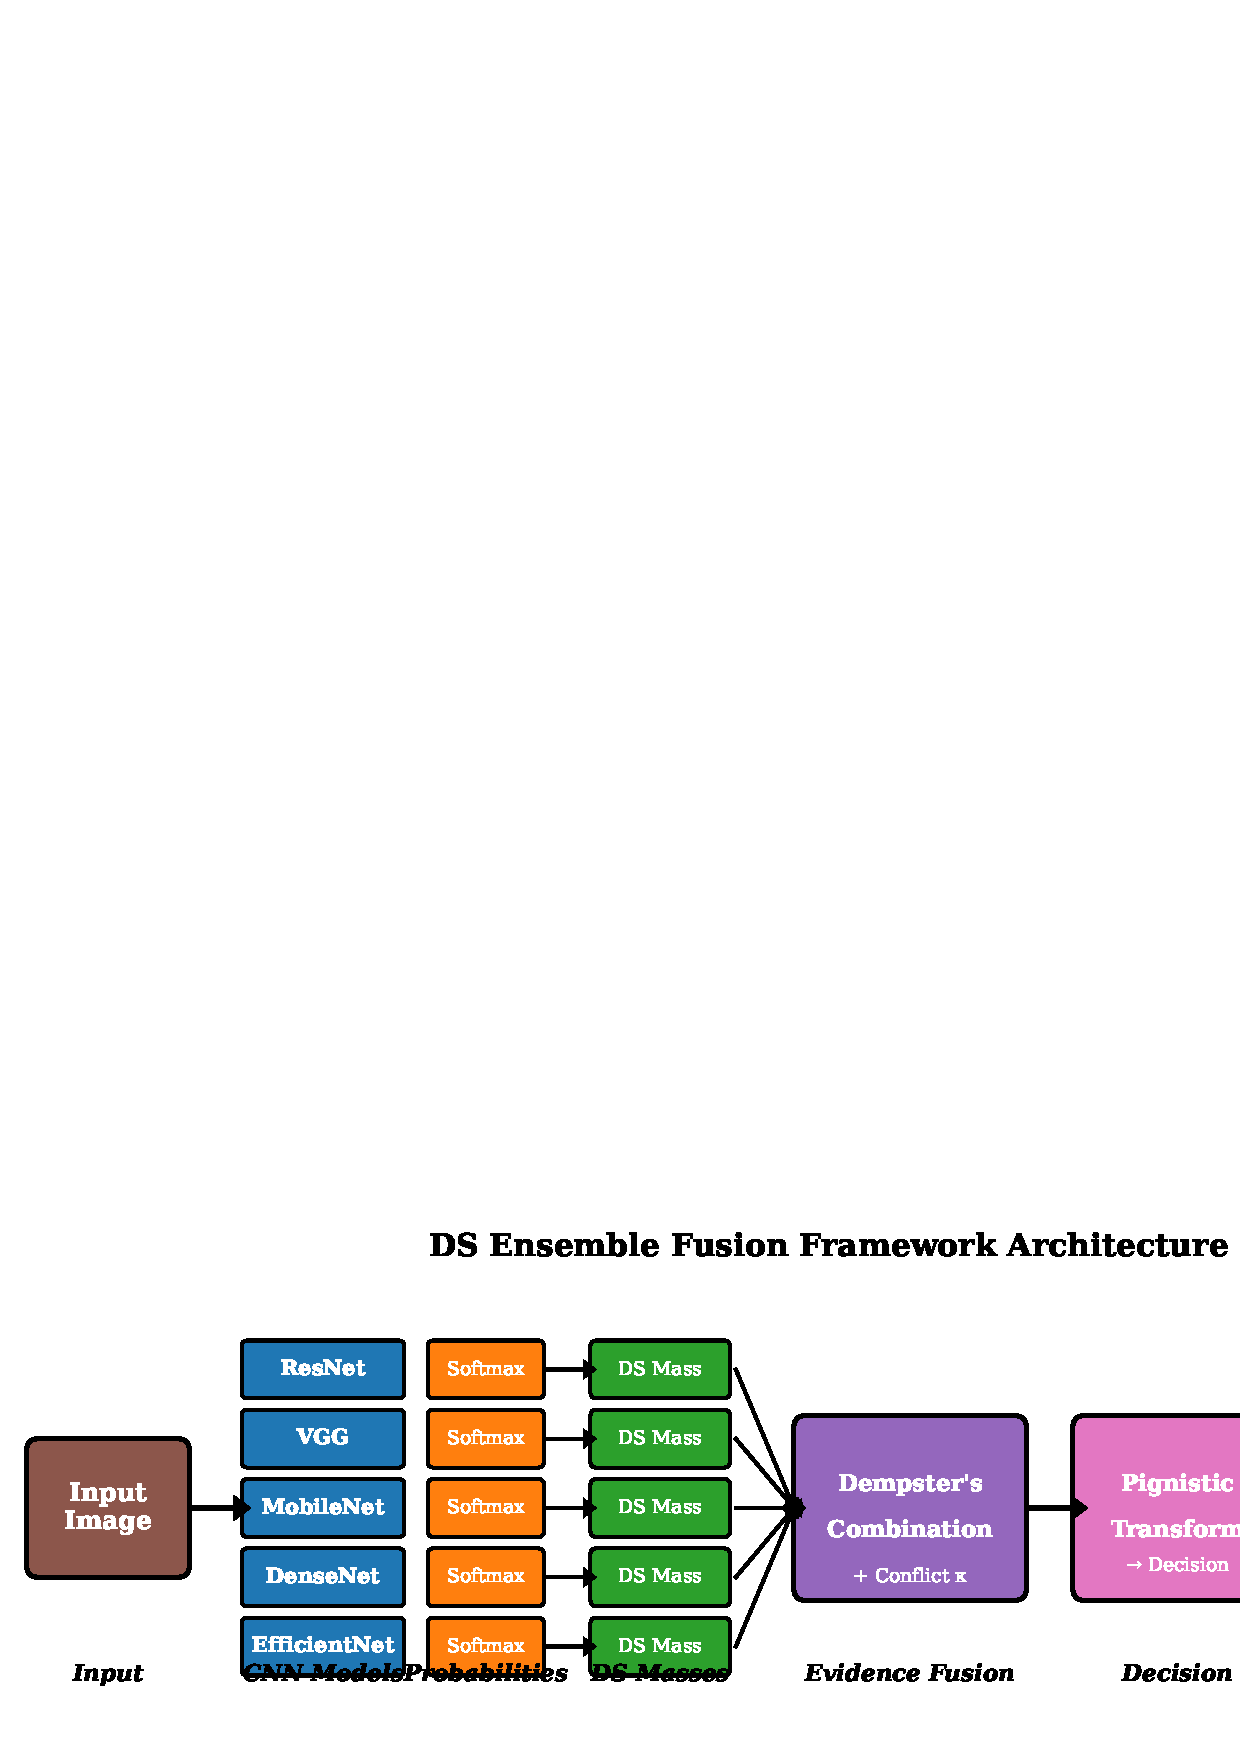
\includegraphics[width=0.95\textwidth]{../results/figures/framework_diagram_polished.png}
\caption{Overview of our DS-based ensemble fusion framework. Individual CNN models generate softmax predictions, which are converted to belief mass functions. These masses are combined using Dempster's rule to produce a fused prediction with explicit uncertainty quantification including belief, plausibility, and conflict measures.}
\label{fig:framework}
\end{figure*}

Each component is designed to preserve the strengths of deep learning (representation power and accuracy) while adding the benefits of DS theory (uncertainty quantification and conflict detection). The framework is model-agnostic and can incorporate any neural network architecture that produces probabilistic outputs.

\subsection{Belief Assignment from Neural Networks}

Given a neural network classifier that outputs softmax probabilities $\mathbf{p} = [p_1, p_2, \ldots, p_K]$ for $K$ classes, we convert these to a DS mass function $m: 2^\Theta \rightarrow [0,1]$, where $\Theta = \{c_1, c_2, \ldots, c_K\}$ is the frame of discernment (set of all classes).

We propose three assignment strategies:

\textbf{Direct Assignment}: The simplest approach directly maps probabilities to mass:
\begin{equation}
m(\{c_i\}) = p_i, \quad \forall i \in \{1, \ldots, K\}
\end{equation}

\textbf{Temperature-Scaled Assignment}: To adjust confidence levels, we apply temperature scaling:
\begin{equation}
m(\{c_i\}) = \frac{\exp(\log p_i / T)}{\sum_{j=1}^K \exp(\log p_j / T)}
\end{equation}
where $T$ is the temperature parameter. $T < 1$ makes the distribution sharper (more confident), while $T > 1$ makes it smoother (less confident).

\textbf{Calibrated Assignment}: Based on model calibration, we adjust the assignment to account for overconfidence:
\begin{equation}
m(\{c_i\}) = \sqrt{p_i} / \sum_{j=1}^K \sqrt{p_j}
\end{equation}

In all cases, any remaining mass (due to normalization or deliberate discount) is assigned to the frame of discernment $\Theta$:
\begin{equation}
m(\Theta) = 1 - \sum_{i=1}^K m(\{c_i\})
\end{equation}
representing ignorance or lack of evidence.

\subsection{Dempster's Rule of Combination}

Given mass functions $m_1$ and $m_2$ from two independent sources, Dempster's rule combines them:
\begin{equation}
m_{1 \oplus 2}(A) = \frac{1}{1-\kappa} \sum_{B \cap C = A} m_1(B) m_2(C)
\end{equation}
where $\kappa$ is the conflict mass:
\begin{equation}
\kappa = \sum_{B \cap C = \emptyset} m_1(B) m_2(C)
\end{equation}

The conflict $\kappa \in [0,1]$ measures disagreement between sources. High conflict indicates contradictory evidence.

For multiple sources $m_1, m_2, \ldots, m_N$, we apply the rule sequentially:
\begin{equation}
m_{combined} = m_1 \oplus m_2 \oplus \cdots \oplus m_N
\end{equation}

\subsection{Uncertainty Metrics}

For a hypothesis $A \subseteq \Theta$, we compute:

\textbf{Belief}: Lower probability bound
\begin{equation}
Bel(A) = \sum_{B \subseteq A} m(B)
\end{equation}

\textbf{Plausibility}: Upper probability bound
\begin{equation}
Pl(A) = \sum_{B \cap A \neq \emptyset} m(B)
\end{equation}

\textbf{Doubt}: Complement of plausibility
\begin{equation}
Doubt(A) = 1 - Pl(A)
\end{equation}

\textbf{Uncertainty Interval}: The interval $[Bel(A), Pl(A)]$ captures prediction uncertainty. A wider interval indicates higher uncertainty.

\subsection{Decision Making}

To make a final prediction, we use the pignistic transformation~\cite{smets1994transferable}, which converts mass to probability:
\begin{equation}
P(c_i) = \sum_{A: c_i \in A} \frac{m(A)}{|A|}
\end{equation}

The predicted class is:
\begin{equation}
\hat{y} = \arg\max_{c_i} P(c_i)
\end{equation}

Alternatively, we can use:
\begin{itemize}
\item \textbf{Maximum Belief}: $\arg\max_{c_i} Bel(\{c_i\})$ (conservative)
\item \textbf{Maximum Plausibility}: $\arg\max_{c_i} Pl(\{c_i\})$ (optimistic)
\end{itemize}

\subsection{Adaptive Weighting}

For models with different reliabilities, we apply discount factors $\alpha_i \in [0,1]$ before fusion:
\begin{equation}
m_i'(A) = (1 - \alpha_i) m_i(A), \quad m_i'(\Theta) = m_i(\Theta) + \alpha_i (1 - m_i(\Theta))
\end{equation}
where $\alpha_i$ represents the unreliability of model $i$.

We can estimate $\alpha_i$ from validation performance:
\begin{equation}
\alpha_i = 1 - \text{Accuracy}_i
\end{equation}

This ensures that less reliable models contribute less mass to specific hypotheses and more to the ignorance set $\Theta$.
